\section{Evaluation}
\label{sec:eval}

We evaluate \sys using four key questions:

\begin{itemize}[leftmargin=*]
  \item \textbf{RQ1 (Single-Tenant Memory/Scheduling):} How much performance gain can \sys's programmable memory and scheduling policies provide on oversubscribed single-tenant workloads?
  \item \textbf{RQ2 (Multi-Tenant Management):} Does \sys's cross-layer policy framework improve tail latency, throughput, and resource fairness compared to user-space and global policies in multi-tenant settings?
  \item \textbf{RQ3 (Programmability \& Generality):} Is \sys sufficiently programmable and general to support diverse resource management policies without significant complexity?
  \item \textbf{RQ4 (Mechanism Overhead):} What is the overhead of \sys's core mechanisms, including its observability capabilities and device-side extensions?
\end{itemize}

\subsection{Methodology and Setup}

We evaluated \sys on two machines. Server~A is a single-socket Intel Core
Ultra~9 285K processor (24 cores) with 128~GB DDR5 RAM and an NVIDIA RTX~5090
GPU. Server~B is a single-socket Intel Xeon~6787P (86~cores, 2.0~GHz, 336~MB
LLC) with 768~GB DDR5 RAM (512~GB CXL module) and an NVIDIA H100 GPU. Unless
otherwise noted, we report results on Server~A and average each metric over
10 trials; when averaging speedups we use geometric means. We compare against
NVIDIA's CUPTI and NVTX-based profiler stack, NVBit gpumemtrace, default UVM
memory management, and the native GPU scheduler without \sys-based policies, as
well as framework-managed offloading where applicable.

\subsubsection{Application workloads}
\label{sec:eval-app-workloads}

We use four unmodified GPU applications from pre-release to evaluate \sys under realistic
end-to-end workloads. In all cases, \sys attaches via runtime and kernel driver
instrumentation; application and framework binaries are unchanged and does not require recompilation.

\paragraph{PyTorch.}
We use PyTorch for both inference and training workloads. For RQ4, we run a ResNet model on ImageNet-sized batches to measure end-to-end inference latency under \sys and the PyTorch profiler (CUPTI+NVTX). For RQ1, we use PyTorch-based GNN training under 1.5$\times$ GPU memory oversubscription to study the impact of programmable UVM policies on epoch time. \sys is loaded as a runtime extension and instruments CUDA kernels without changes to the PyTorch code, models, or training loops.

\paragraph{\texttt{llama.cpp}.}
We use the GPT-OSS-120B configuration in \texttt{llama.cpp} to evaluate expert offload policies (RQ1). The model is approximately 60~GB on an RTX~5090 with 32~GB of device memory, so inference runs in oversubscribed mode with UVM and the framework's built-in offload support. \sys attaches transparently at the driver level and via device-side handlers that tag expert regions as ``hot'' or ``cold'' and drive prefetch/eviction decisions.

\paragraph{vLLM.}
We evaluate vLLM on a 30B FP8 MoE model to study KV-cache placement and offloading policies (RQ1) under realistic serving loads. We use a ShareGPT benchmark with 100 requests and around 30 concurrent requests to stress KV-cache growth and reuse. \sys runs alongside vLLM with UVM enabled and implements sequential prefetch and eviction policies for KV-cache segments via callbacks and GPU handlers.

\paragraph{Faiss.}
We integrate \sys with the GPU backend of Faiss to evaluate vector search with oversubscribed indices (RQ1). We consider both index build and query workloads where the index does not fit in device memory and UVM migrates index pages over PCIe. \sys observes and steers index-segment placement by instrumenting GPU memory operations and monitoring PCIe traffic, keeping frequently accessed centroids and posting lists resident while demoting cold segments.

\subsection{RQ1: Single-Tenant Memory and Scheduling Policies}

We evaluate \sys's memory policy interface on the application workloads introduced in Section~\ref{sec:eval-app-workloads}, focusing on oversubscribed single-tenant setups where memory placement and prefetching dominate performance.

\paragraph{Expert Offloading (llama.cpp GPT-OSS-120B).}
For the GPT-OSS-120B model in \texttt{llama.cpp}, a \sys policy that triggers a
max-prefetch strategy on GPU-side memory events (prefetching additional experts
when entering an expert region and evicting based on expert-level hotness)
improves throughput by up to 5$\times$ compared to default UVM and the
framework's own offloading, under the oversubscribed configuration described in
Section~\ref{sec:eval-app-workloads}. This policy is expressed as eBPF callbacks
in the driver plus device-side handlers that mark expert regions as
``will-use soon'' or ``cold'' without modifying the application.

\begin{figure}
\centering
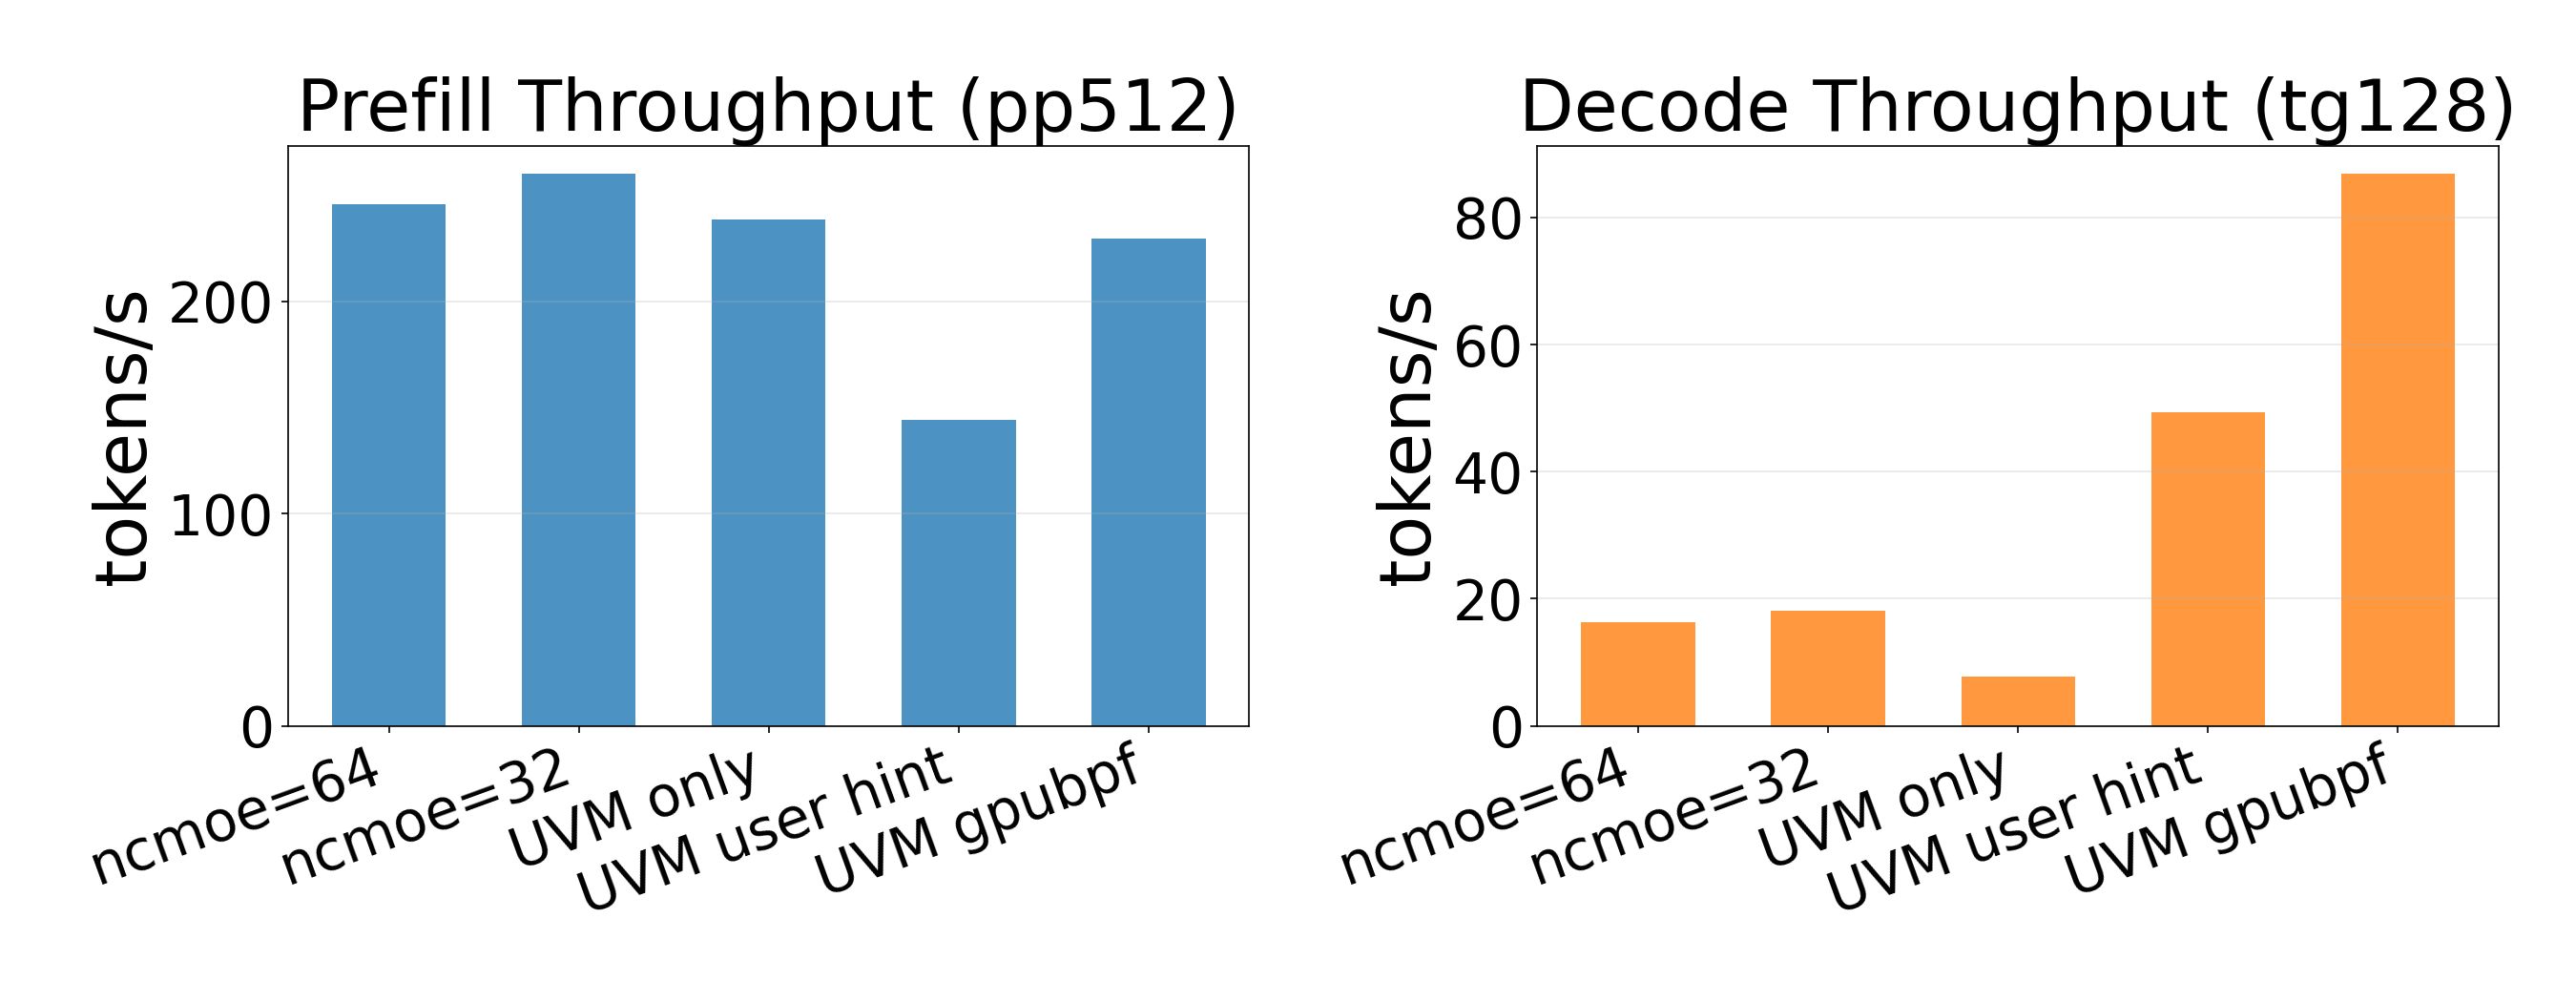
\includegraphics[width=\columnwidth]{img/results-raw/llama.cpp/llama_uvm_combined_color.png}
\caption{Throughput of \sys expert-region caching policy vs default UVM and llama.cpp offloading across varying oversubscription ratios (model 60GB, GPU 32GB).}
\label{fig:llama-expert-offload}
\end{figure}

% TODO: Add mechanism figure - per-miss stall CDF or timeline explaining where 5x comes from (fewer faults + bulk prefetch)
\begin{figure}
\centering
\fbox{\parbox{\columnwidth}{\centering [Figure: llama.cpp Timeline/CDF - Mechanism Analysis]}}
\caption{Per-miss stall timeline showing reduction in GPU stall time due to optimized bulk-prefetch decisions driven by GPU-side execution hints.}
\label{fig:llama-mechanism}
\end{figure}

\paragraph{KV-cache Offloading (vLLM Qwen-30B MoE).}
We evaluate on the Qwen-30B FP8 MoE model ($\approx$30GB) on RTX 5090 (32GB). The model alone nearly fills GPU VRAM, so default no-offload configuration OOMs under load. We stress KV-cache growth by sending 100 concurrent requests from ShareGPT (single-round, no prefix caching), resulting in total memory footprint of 36--40GB (model + KV-cache for $\approx$60K tokens aggregate). Existing solutions typically offload either KV-cache or MoE experts, but not both; in contrast, UVM attempts on-demand migration of both, leading to thrashing.

We compare vLLM's CPU-offload mode (\texttt{--cpu-offload-gb 8}) against \sys with UVM and a simple sequential prefetch policy based on PCIe traffic patterns. This policy performs more aggressive prefetching than fixed heuristics, reducing thrashing and page faults. \sys improves mean and p99 time-to-first-token by 1.7--2$\times$ and decoding throughput by about 1.3$\times$ over vLLM's framework-managed offload (\Cref{fig:vllm-kv-offload}). Simply enabling UVM without \sys policies performs worse than vLLM's own offload; the \sys configuration is roughly 2--3$\times$ faster than this UVM-only baseline. This demonstrates that \sys's programmable driver-level policies can match or exceed SOTA framework-managed offloading while providing better p99 latency, even in single-tenant scenarios.

\begin{figure}
\centering
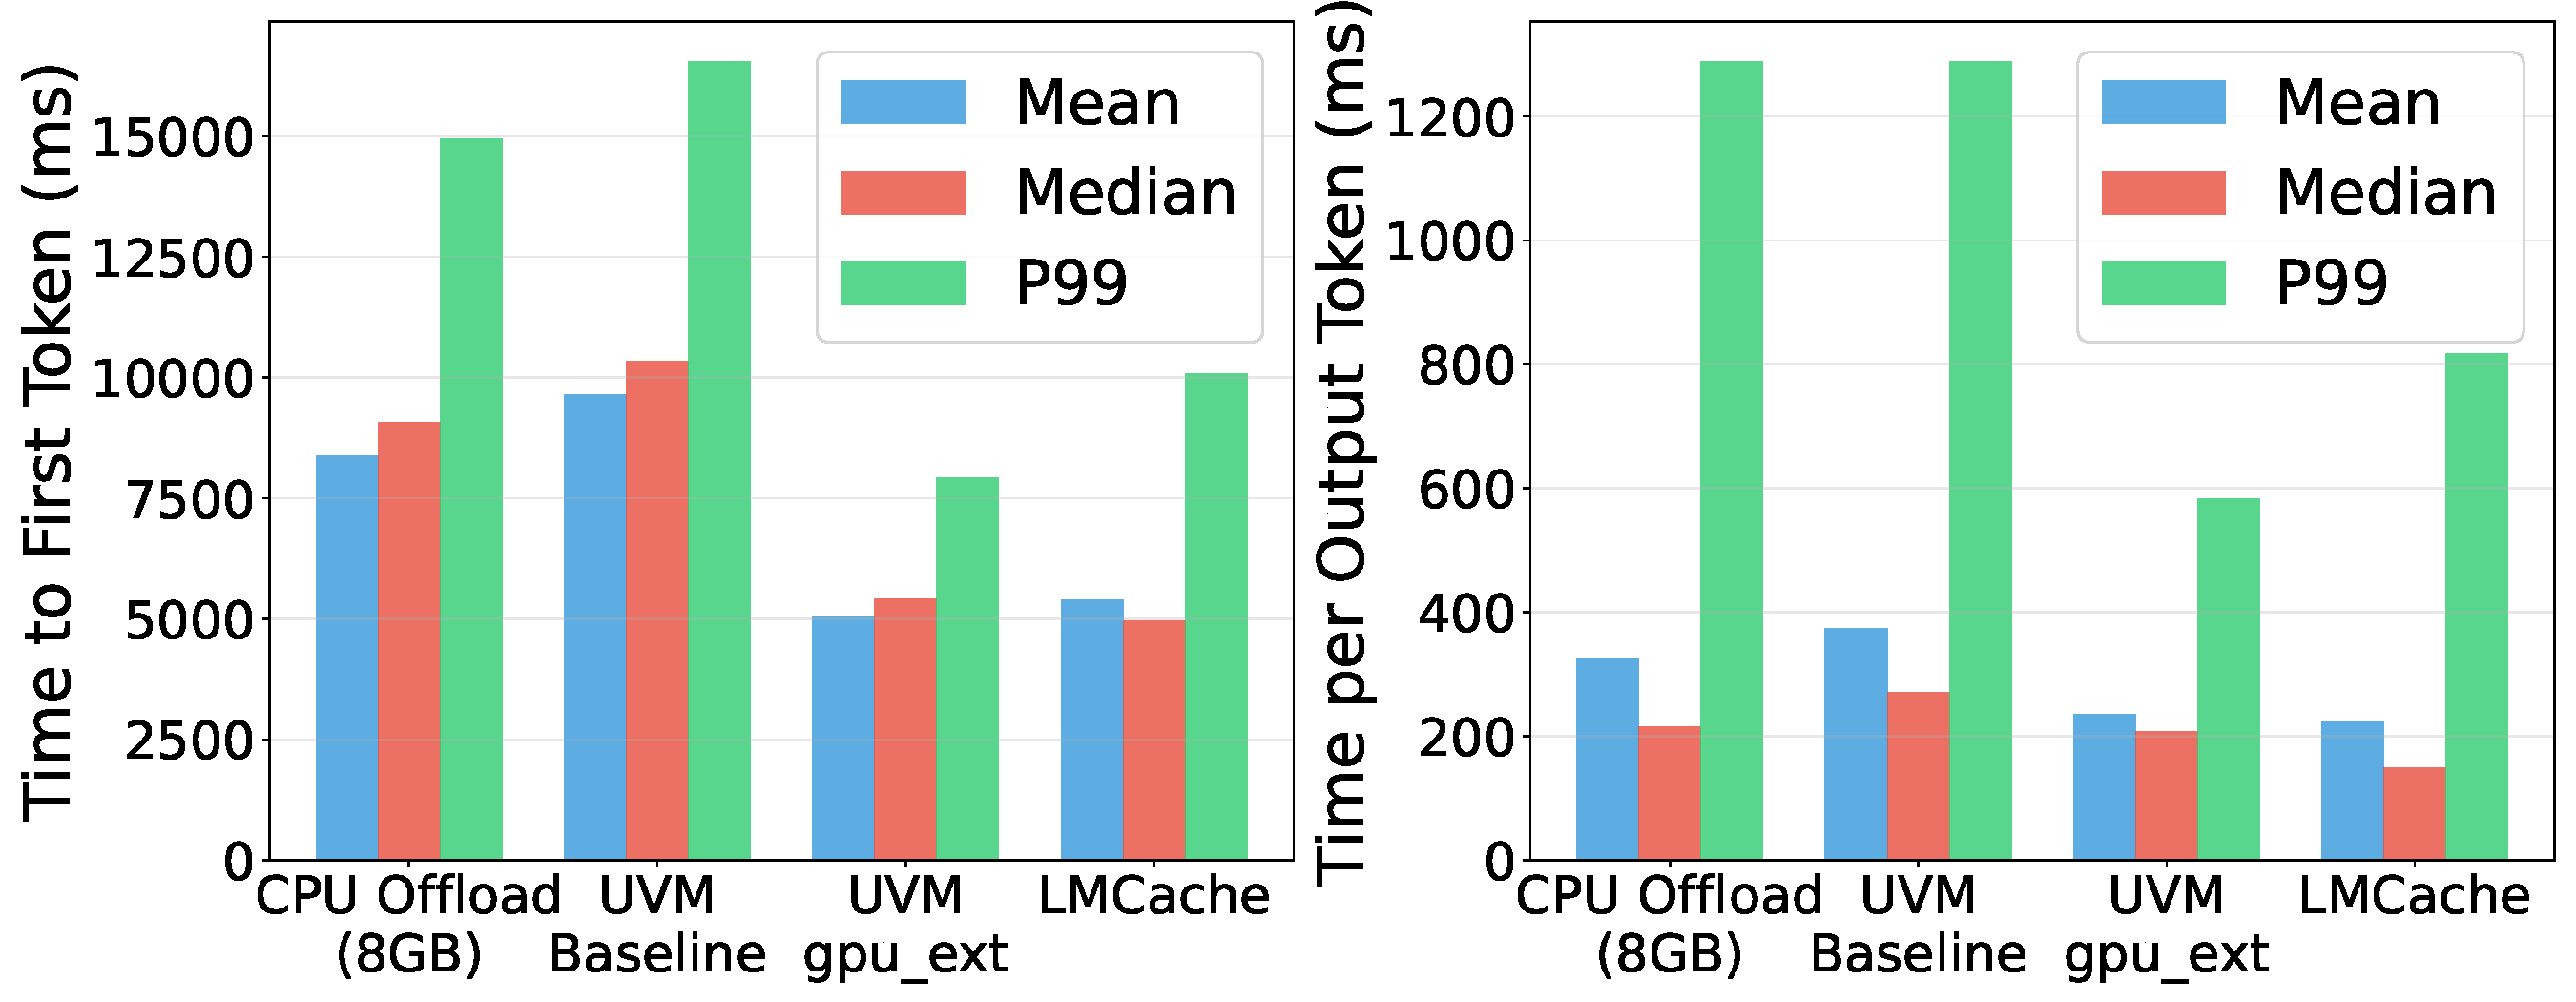
\includegraphics[width=\columnwidth]{img/results-raw/vllm/ttft_tpot_combined.pdf}
\caption{Time-to-first-token and decoding throughput for \sys KV-aware sequential prefetch policy vs vLLM CPU-offload on Qwen-30B FP8 MoE with 100 concurrent requests ($\approx$60K tokens KV-cache).}
\label{fig:vllm-kv-offload}
\end{figure}

\paragraph{Graph Neural Networks (GNN Training).}
For GNN workloads, we run PyTorch-based training under 1.5$\times$
oversubscription of GPU memory. With default UVM, epoch time is around 71~s.
With a simple \sys policy that performs sequential prefetching of adjacency and
feature blocks and FIFO-style eviction, average epoch time drops to about 26~s,
a 2--3$\times$ improvement. For comparison, the same training job with a 0.8$\times$
working set that fits entirely in GPU memory completes an epoch in 15~s; \sys
thus brings the oversubscribed configuration close to the non-oversubscribed
baseline. The CPU-side framework overhead for these policies is around 1\%, and
device-side instrumentation adds 2--3\%.

\begin{figure}
\centering
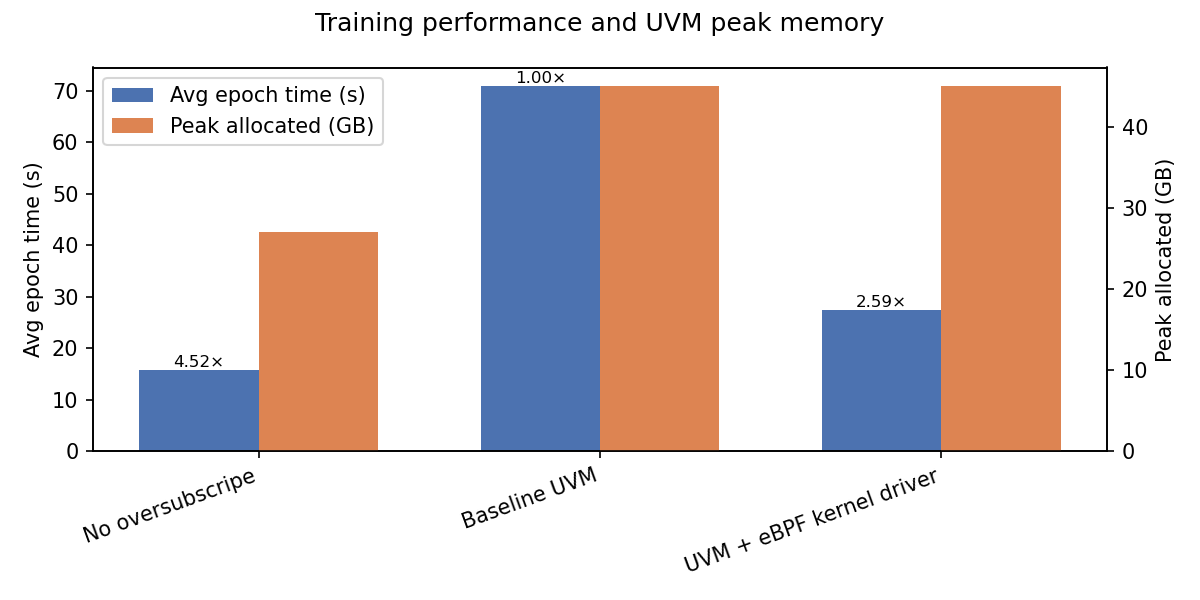
\includegraphics[width=\columnwidth]{img/results-raw/pytorch/uvm_perf_vs_memory.png}
\caption{Epoch time for GNN training with 1.5$\times$ GPU memory oversubscription: fit-in-HBM (15s), default UVM (71s), and \sys block-level prefetch with FIFO eviction (26s).}
\label{fig:gnn-epoch}
\end{figure}

\paragraph{Faiss Vector Search.}
For Faiss, a \sys policy that adaptively prefetches index segments based
on observed PCIe traffic and access streams reduces index build time by about
1.5$\times$ compared to default UVM behavior when the index does not fit in
device memory. Query workloads see similar benefits from keeping frequently
accessed centroids and posting lists resident and demoting cold segments.

\begin{figure}
\centering
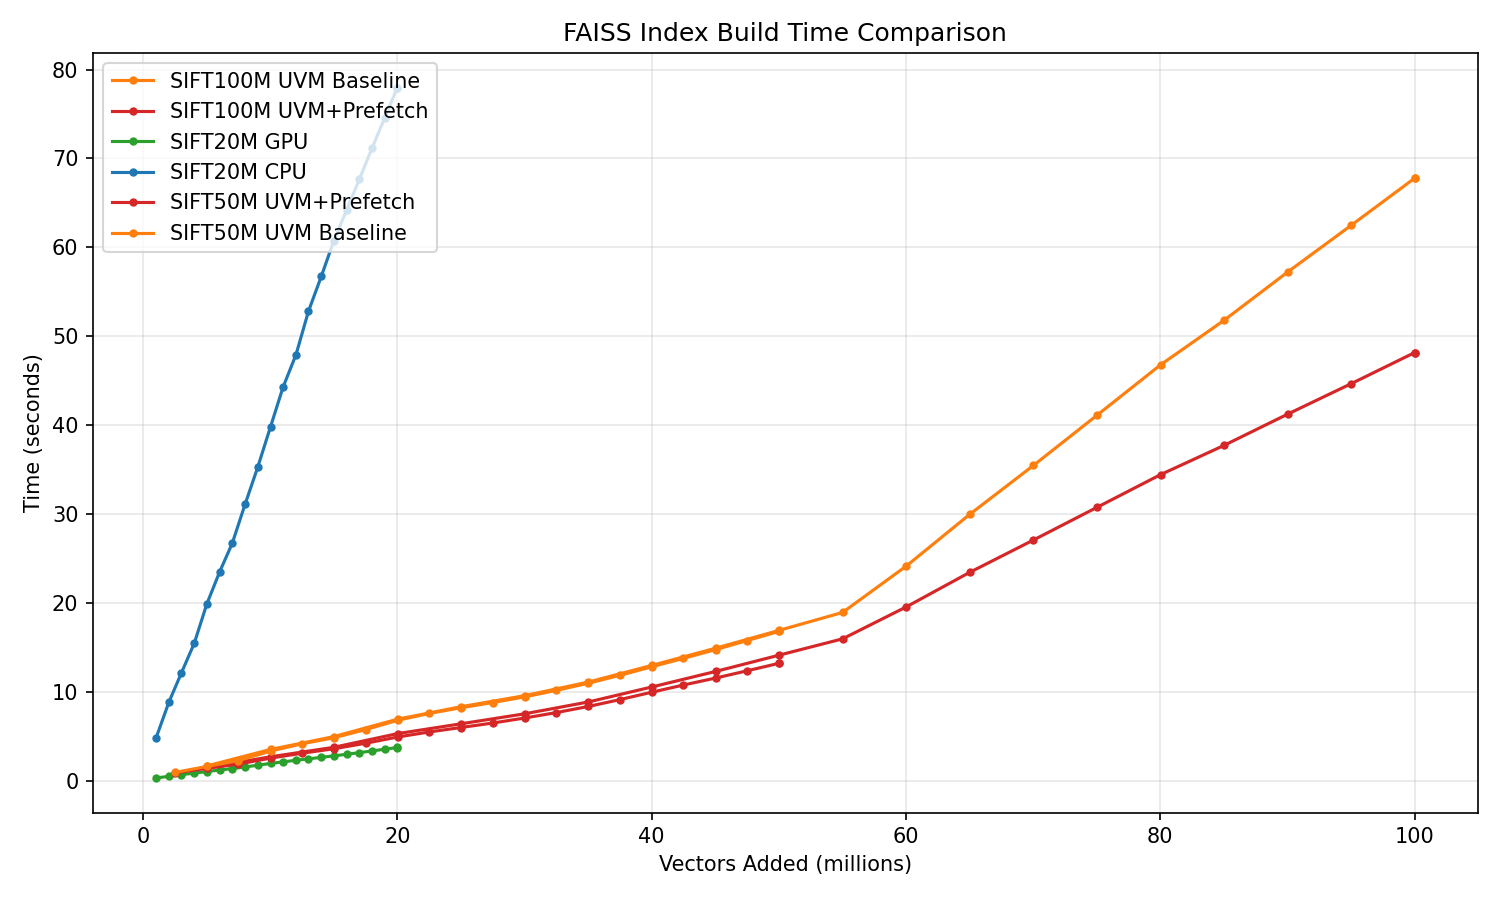
\includegraphics[width=\columnwidth]{img/results-raw/faiss/faiss_buildindex.png}
\caption{Faiss index build time and query throughput with \sys adaptive prefetch policy vs default UVM under oversubscribed index segments ($\approx$1.5$\times$ speedup).}
\label{fig:faiss-perf}
\end{figure}

\paragraph{Single-Tenant Block Scheduler.}
We apply a \sys-based block scheduler driven by the GPU-side interface
(Section~\ref{sec:design-sched}) to workloads with significant load imbalance.
Using a cluster-style launch where persistent worker blocks pull work units
via \texttt{should\_try\_steal}, we evaluate on AI inference with dynamic batching
and GEMM with variable matrix sizes where static block assignment leads to some blocks being overloaded while others idle.

\Cref{fig:block-scheduler-single} compares three scheduling policies: FixedWork (static block assignment), CLC Baseline (cooperative launch control), and workload-aware policies (WorkloadAware for inference, TokenBucket for GEMM). On AI inference with dynamic batching, the workload-aware policy reduces execution time from 27~µs (FixedWork) to 17~µs, a 37\% improvement. On imbalanced GEMM, TokenBucket achieves 51~µs compared to 67~µs for FixedWork, a 24\% improvement across variable MxNxK configurations.

\begin{figure}
\centering
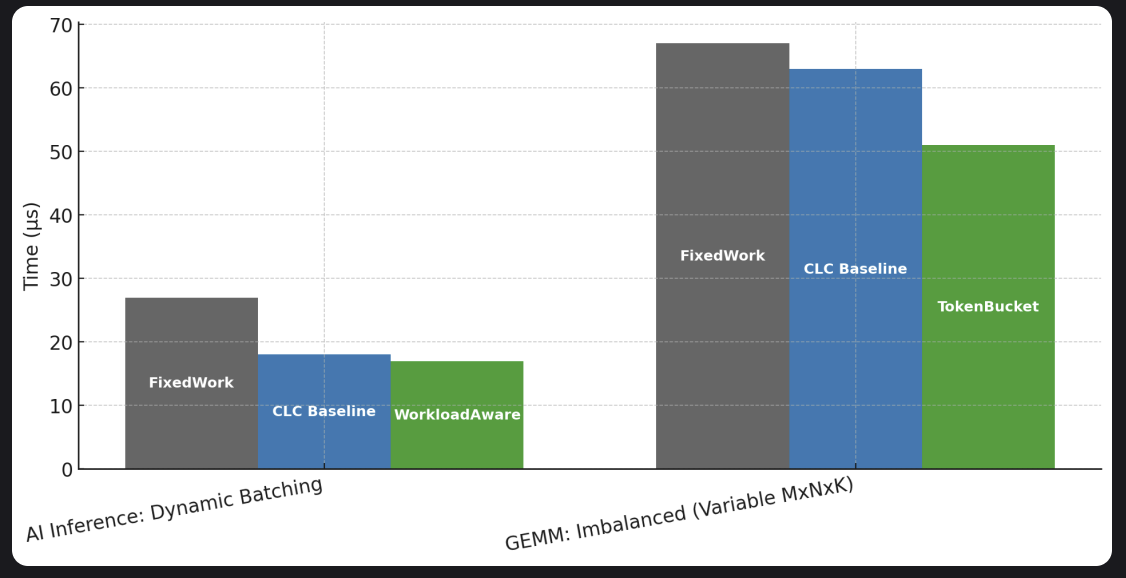
\includegraphics[width=\columnwidth]{img/results-raw/sync/clc/clc-policy.png}
\caption{Block scheduler performance on load-imbalanced workloads: AI inference with dynamic batching and GEMM with variable matrix sizes. Workload-aware \sys policies achieve 24--37\% improvement over static assignment.}
\label{fig:block-scheduler-single}
\end{figure}

Across these applications, the common pattern is that programmable region-based
placement and prefetch policies in \sys allow the system to exploit workload
structure (experts, KV-cache, graph structure, index layout) that existing UVM
policies and framework-level offload mechanisms cannot leverage without invasive
changes.

\subsection{RQ2: Multi-Tenant Memory, Bandwidth, and Scheduling}

We evaluate \sys's cross-layer policy framework on multi-tenant GPU workloads, comparing per-tenant policies against global policies and framework-managed approaches. We focus on tail latency, throughput, resource fairness, and GPU utilization.

\paragraph{Two-Tenant: High-Priority LLM + Background GNN/Faiss.}
We run two tenants sharing a single GPU and host/CXL memory: T1 is a high-priority vLLM chat service (short context, p99 SLA), and T2 is background GNN training or Faiss query (latency-insensitive). We compare three policy configurations: (1) global FIFO/LRU (driver default + UVM), (2) framework-managed policies (vLLM CPU-offload + GNN prefetch, operating in separate planes), and (3) \sys per-tenant policies where each tenant has its own HBM credit and bandwidth budget, with eviction/prefetch hooks respecting tenant quotas and the scheduler prioritizing T1.

% TODO: Add experiment data
% Metrics: T1 p50/p95/p99 (normalized by solo), T2 throughput, GPU utilization
% Target: per-tenant gBPF => T1 p99 ~ solo, T2 throughput near baseline
\begin{figure}
\centering
\fbox{\parbox{\columnwidth}{\centering [Figure: Two-Tenant Policy Comparison - T1 p99, T2 Throughput, GPU Util]}}
\caption{Two-tenant (high-priority LLM + background GNN) performance under global FIFO/LRU, framework-managed, and \sys per-tenant policies. \sys achieves near-solo p99 for T1 (within TODO\%) while maintaining T2 throughput (TODO\% of baseline).}
\label{fig:two-tenant}
\end{figure}

\paragraph{Three-Tenant: LLM + LLM + Faiss (KV + Bandwidth Contention).}
We evaluate a more LLM-centric multi-tenant scenario with three tenants: T1 (short-context chat, high priority), T2 (long-context LLM, KV-heavy), and T3 (Faiss vector search, latency-sensitive but can tolerate some degradation). Baseline uses each runtime's offload mechanism plus default UVM. \sys implements per-tenant KV region cache, bandwidth budgets, and priority scheduling.

% TODO: Add experiment data
% Metrics: per-tenant p99/throughput, cross-tenant p99 inflation (p99_shared/p99_solo)
\begin{figure}
\centering
\fbox{\parbox{\columnwidth}{\centering [Figure: Three-Tenant p99 Inflation and GPU Utilization]}}
\caption{Three-tenant (LLM chat + LLM long-context + Faiss) p99 latency inflation (p99\_shared / p99\_solo) under baseline vs \sys per-tenant policies. TODO: specific numbers.}
\label{fig:three-tenant}
\end{figure}

\paragraph{Priority Scheduler (Real-time + Batch).}
We evaluate \sys's priority scheduling on mixed multi-tenant workloads combining real-time video processing kernels (high priority) with batch ML training (low priority). We compare three approaches: (1) no prioritization (FIFO), (2) CUDA stream-level priorities, and (3) \sys-based priority scheduling with warp-level preemption.

\Cref{fig:p99-latency} plots p99 latency for high-priority tasks. FIFO exhibits 25--80~ms p99 latency due to blocking behind long-running kernels. CUDA streams reduce p99 to 15--30~ms but still suffer head-of-line blocking. \sys cuts p99 latency to 5--12~ms by preempting low-priority warps at synchronization points and admitting high-priority kernels promptly. Scheduling decisions take 0.3--0.8~µs with 4--6\% overhead.

\begin{figure}
\centering
\fbox{\parbox{\columnwidth}{\centering [Figure: Priority Scheduler Tail Latency]}}
\caption{p99 latency for high-priority tasks under FIFO, CUDA stream priorities, and \sys warp-level preemption in multi-tenant scheduling.}
\label{fig:p99-latency}
\end{figure}

\Cref{fig:lowprio-throughput} shows the impact on low-priority throughput. \sys incurs an 8--12\% throughput reduction compared to FIFO due to preemption overheads, but maintains better fairness than CUDA streams, which reduce low-priority throughput by 18--25\% and can starve low-priority work for long intervals.

\begin{figure}
\centering
\fbox{\parbox{\columnwidth}{\centering [Figure: Low-Priority Task Throughput]}}
\caption{Throughput impact on low-priority tasks with different scheduling policies in multi-tenant scenarios.}
\label{fig:lowprio-throughput}
\end{figure}

Overall, \sys's per-tenant policies provide clear tail-latency and fairness benefits in multi-tenant workloads, achieving near-solo performance for high-priority tenants while maintaining reasonable throughput for background jobs.

\subsection{RQ3: Programmability and Generality}

We evaluate \sys's programmability by examining policy complexity (lines of code), support across diverse workloads, and the relationship between policy complexity and runtime overhead.

\paragraph{Support Matrix.}
\Cref{tab:support-matrix} shows the policies implemented for each workload, along with lines of code (host eBPF + device eBPF) and measured overhead. All policies attach to unmodified frameworks via \sys's runtime instrumentation. The key takeaway is that a few hundred lines of policy code can implement sophisticated cross-layer resource management without application changes.

% TODO: Fill in actual LOC and overhead numbers
\begin{table}[t]
\centering
\small
\caption{Policy support matrix across workloads. LOC = host eBPF + device eBPF lines.}
\label{tab:support-matrix}
\begin{tabular}{lcccc}
\toprule
\textbf{Workload} & \textbf{Observability} & \textbf{Memory} & \textbf{Scheduling} & \textbf{Overhead} \\
\midrule
PyTorch ResNet & threadhist, mem\_trace & -- & -- & 2--3\% \\
PyTorch GNN & kernelretsnoop & block prefetch (TODO LOC) & -- & 2--3\% \\
llama.cpp 120B & launchlate & expert cache (TODO LOC) & block sched (TODO LOC) & 3--4\% \\
vLLM 30B & mem\_trace & KV prefetch (TODO LOC) & priority (TODO LOC) & 2--3\% \\
Faiss & kernelretsnoop & segment cache (TODO LOC) & -- & 2--3\% \\
\bottomrule
\end{tabular}
\end{table}

\paragraph{Policy Complexity vs Overhead.}
\Cref{fig:complexity-overhead} plots policy complexity (approximated by eBPF instruction count, map operations, and helper calls) against runtime overhead measured on a standard workload. Even complex tenant-aware policies incur less than 5\% overhead, demonstrating that \sys's design scales gracefully with policy sophistication.

% TODO: Add actual data points
% x-axis: policy complexity (instruction count / map ops / helper calls)
% y-axis: overhead (%)
% Points: observability tools, simple memory policy, tenant-aware policy, priority scheduler, block scheduler
\begin{figure}
\centering
\fbox{\parbox{\columnwidth}{\centering [Figure: Policy Complexity vs Overhead Scatter Plot]}}
\caption{Policy complexity vs runtime overhead. Observability tools (mem\_trace, threadhist) cluster at low complexity/overhead; tenant-aware memory and scheduling policies remain under 5\% overhead despite higher complexity.}
\label{fig:complexity-overhead}
\end{figure}

\paragraph{Policy Reuse Across Workloads.}
The region cache policy skeleton used for llama.cpp expert offloading can be adapted to vLLM KV-cache management by changing only the region identification helpers and ID mappings. Similarly, the sequential prefetch policy applies to both GNN adjacency blocks and Faiss index segments with minimal modification (TODO: X lines changed out of Y total). This demonstrates \sys's support for portable, reusable policy components.

\subsection{RQ4: Runtime Overhead and Observability}

We evaluate the efficiency of \sys's core mechanisms and its observability capabilities. We first quantify the base runtime overhead and shared state costs, then demonstrate that \sys enables practical observability tools with significantly lower overhead than existing frameworks.

\subsubsection{Runtime and Shared State Overhead}

We first quantify the overhead of the \sys runtime itself, independent of any
specific policy logic. We use two microbenchmarks:

\begin{itemize}[leftmargin=*]
  \item a load/store latency benchmark that issues controlled memory accesses
        from GPU kernels, instrumented with \sys and with NVBit gpumemtrace; and
  \item a ResNet inference workload instrumented with \sys-based tracing and
        with the PyTorch profiler (CUPTI+NVTX).
\end{itemize}

\Cref{fig:runtime-overhead} shows per-access latency slowdown under
\sys and NVBit as access sizes increase. \sys adds substantially less latency
than NVBit, remaining low and stable below 128~KB and increasing modestly
thereafter. \Cref{fig:resnet-latency} compares end-to-end ResNet inference
latency distributions: p10 and mean latencies under \sys are slightly better
than with the PyTorch profiler, and p99 latency is comparable. In both cases,
lightweight launch-time injection and warp-level execution of \sys handlers
keep overhead low.

\begin{figure}
\centering
\fbox{\parbox{0.5\textwidth}{\centering [Figure: Runtime Overhead]}}
\caption{Runtime overhead of \sys vs NVBit across varying access sizes.}
\label{fig:runtime-overhead}
\end{figure}

\begin{figure}
\centering
\fbox{\parbox{0.5\textwidth}{\centering [Figure: Resnet Inference Latency Overhead]}}
\caption{ResNet inference latency with \sys tracing vs PyTorch profiler (CUPTI+NVTX).}
\label{fig:resnet-latency}
\end{figure}

\paragraph{Map and Shared State Overhead.}
We measure the cost of maintaining shared state between CPU and GPU via \sys maps (\Cref{tab:map-overhead}). We benchmark shared-memory bandwidth and one-way latency on both servers using a 1~GiB region and GPU-to-CPU and CPU-to-GPU access patterns. Servers~A and~B deliver 12--18~GB/s over PCIe with 8--15~µs cross-domain latencies. These costs are small relative to the time scales of the policies we implement, and our SIMT-aware aggregation and sampling strategies further reduce the frequency of cross-domain synchronization.

% TODO: Add map size vs overhead microbench if time permits
\begin{table}[t]
\centering
\small
\caption{Shared state (map) overhead for cross-domain communication.}
\label{tab:map-overhead}
\begin{tabular}{lcc}
\toprule
\textbf{Metric} & \textbf{Server A (RTX 5090)} & \textbf{Server B (H100)} \\
\midrule
GPU$\rightarrow$CPU bandwidth & 12--14 GB/s & 16--18 GB/s \\
CPU$\rightarrow$GPU bandwidth & 12--14 GB/s & 16--18 GB/s \\
One-way latency & 10--15 µs & 8--12 µs \\
Map memory overhead & <1\% HBM & <1\% HBM \\
\bottomrule
\end{tabular}
\end{table}

\subsubsection{Low-overhead GPU Observability}

We evaluate the suite of bcc-style observability tools built on \sys, measuring
accuracy, overhead, and practical utility across diverse workloads.

\paragraph{Thread divergence and workload balance.}
\texttt{kernelretsnoop} attaches to kernel return paths and records per-thread
timestamps. Applied to a matrix multiply kernel with boundary checks, it shows
that threads handling edge cases (5\% of total) incur 600--850~ns longer
execution than interior threads, with timestamps within 10~ns of hardware
performance counters and 2.1\% overhead. Refactoring boundary handling based on
this insight improves overall kernel performance by 8\%. \texttt{threadhist}
reveals load imbalance in a particle simulation with 1M particles across 256
blocks: it identifies a bimodal distribution of iterations per thread;
rebalancing particles based on this information yields an 18\% throughput
improvement with 1.8\% tool overhead.

\paragraph{Launch latency and memory behavior.}
\texttt{launchlate} combines host and device hooks to measure kernel launch
latency. On a pipeline of 50 small kernels (each around 100~µs execution time),
default synchronous execution yields 150--550~µs launch latency per kernel, for
a total runtime of 32~ms. Switching to CUDA graphs, guided by
\texttt{launchlate}, reduces this to 7.2~ms, with less than 0.5\% overhead.
\texttt{mem\_trace} instruments sampled memory operations and recovers per-warp
bank conflict rates within 2\% of hardware counters, with under 3\% end-to-end
overhead across GEMM, SpMV and stencil kernels (\Cref{fig:obs-overhead}).

\begin{figure}
\centering
\fbox{\parbox{\columnwidth}{\centering [Figure: GPU Observability Tools Overhead Comparison]}}
\caption{Overhead of \sys-based observability tools across workloads.}
\label{fig:obs-overhead}
\end{figure}

\paragraph{Comparison to CUPTI and NVBit.}
\Cref{fig:obs-comparison} compares \sys-based tools against CUPTI and
NVBit for common profiling tasks. CUPTI-based profiling incurs 15--25\%
overhead and typically requires kernel restarts; NVBit adds 30--45\%
overhead for similar metrics. \sys tools average 2--3\% overhead and support
live instrumentation without interrupting execution.

\begin{figure}
\centering
\fbox{\parbox{\columnwidth}{\centering [Figure: Observability Tool Comparison]}}
\caption{Comparison of \sys observability tools vs CUPTI and NVBit across GEMM, SpMV, and stencil kernels. \sys achieves 2--3\% overhead vs CUPTI 15--25\% and NVBit 30--45\%.}
\label{fig:obs-comparison}
\end{figure}

\paragraph{Device-side Microbenchmarks and Optimization Effects.}
We evaluate device-side \sys mechanisms using a vector-add microbenchmark (32 elements, 10K iterations) on RTX 5090. \Cref{fig:microbench}(a) compares latency before and after our SIMT-aware warp-level execution optimizations (\S\ref{sec:verification}), with a baseline of 5.2~μs. Empty probe latency drops from 6.2~μs to 5.5~μs (-11\%), and exit probe from 6.2~μs to 5.3~μs (-14\%). More complex operations show larger improvements: array map lookup drops from 8.2~μs to 5.8~μs (-30\%), array map update from 11.1~μs to 7.0~μs (-37\%), and Memtrace from 9.4~μs to 6.1~μs (-35\%). \Cref{fig:microbench}(b) shows CPU map access via PCIe incurs ~33,700~μs latency---approximately 6000$\times$ slower than GPU-side operations, motivating \sys's hierarchical map design that keeps hot state on GPU.

\begin{figure*}
\centering
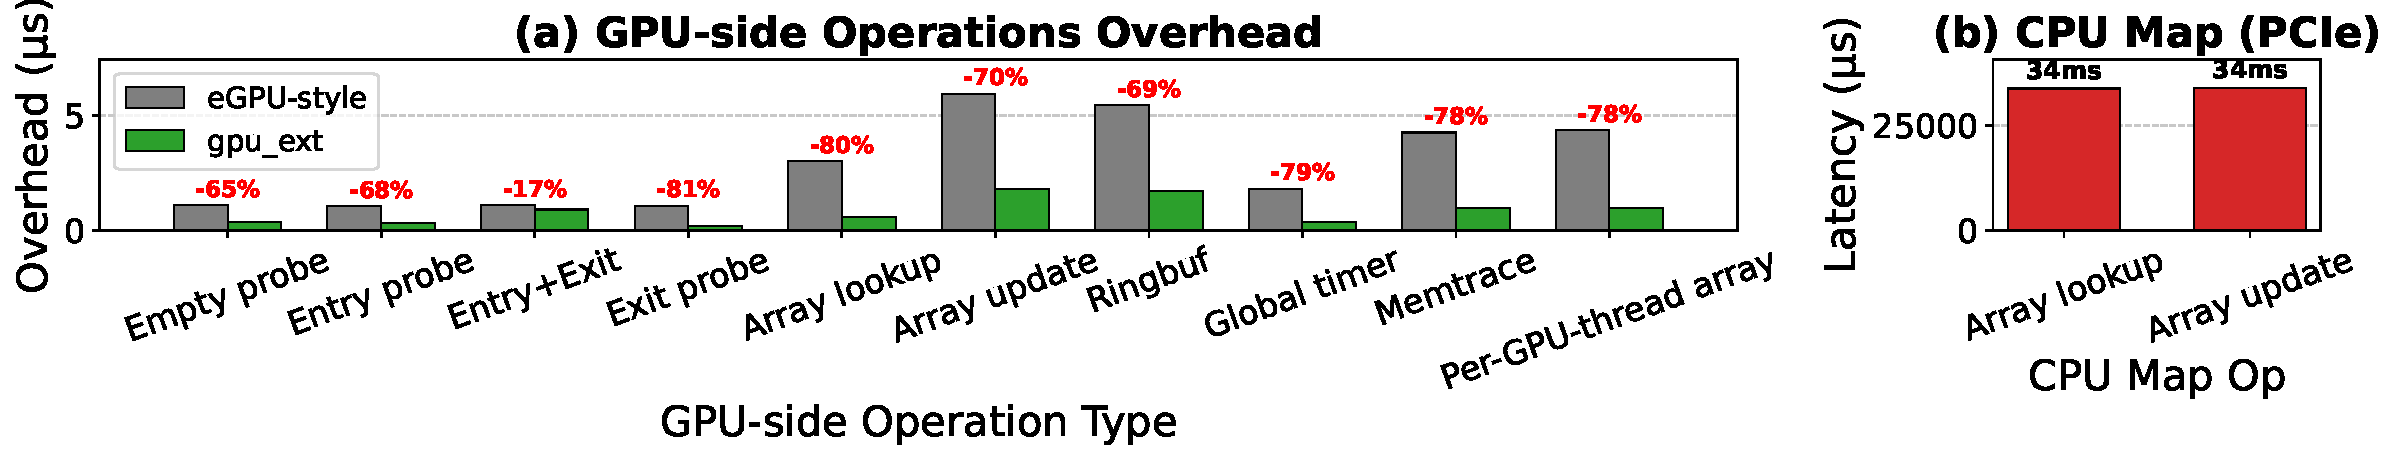
\includegraphics[width=\textwidth]{img/results-raw/runtime/microbench_comparison.pdf}
\caption{Device-side microbenchmark latency. (a) GPU-side operations before/after SIMT-aware optimizations show 11--37\% latency reduction. (b) CPU map access via PCIe is ~6000$\times$ slower than GPU-side operations.}
\label{fig:microbench}
\end{figure*}
